\documentclass[letterpaper,12pt]{report}
\usepackage[pdftex]{graphicx}
\usepackage{setspace}
\usepackage{fullpage}
\usepackage{pdfpages}
\usepackage[titletoc]{appendix}
\usepackage{titlesec}
\usepackage{paralist}
\usepackage{url}
\usepackage{array}
\usepackage{multirow}
\usepackage{rotating}
\usepackage{xparse}

%% Custom C table column type for fixed width
\newcolumntype{C}[1]{>{\let\newline\\\arraybackslash\hspace{0pt}}m{#1}}

% Rotation: \rot[<angle>][<width>]{<stuff>} 
\NewDocumentCommand{\rot}{O{45} O{1em} m}{\makebox[#2][l]{\rotatebox{#1}{#3}}}

%% Adjust title spacing and borders.
\titleformat{\chapter}[display]
{\normalfont\huge\bfseries}{\chaptertitlename\ \thechapter}{20pt}{\Huge}
\titleformat{\section}
{\normalfont\large\bfseries\singlespacing}{\thesection}{1em}{}
\titleformat{\subsection}
{\normalfont\normalsize\bfseries\singlespacing}{\thesubsection}{1em}{}
\titleformat{\subsubsection}
{\normalfont\normalsize\bfseries\singlespacing}{\thesubsubsection}{1em}{}

\titlespacing*{\chapter}{0pt}{5pt}{25pt}
\titlespacing*{\section} {0pt}{3.5ex plus 1ex minus .2ex}{2.3ex plus .2ex}
\titlespacing*{\subsection} {0pt}{3.25ex plus 1ex minus .2ex}{1.5ex plus .2ex}
\titlespacing*{\subsubsection}{0pt}{3.25ex plus 1ex minus .2ex}{1.5ex plus .2ex}

%% Define a new 'leo' style for the package that will use a smaller font.
\makeatletter
\def\url@leostyle{%
  \@ifundefined{selectfont}{\def\UrlFont{\sf}}{\def\UrlFont{\small\ttfamily}}}
\makeatother
%% Now actually use the newly defined style.
\urlstyle{leo}


\title{CLARKSON UNIVERSITY \\
\ \\
Overcoming Geographic Isolation: The Design and Implementation of a Web-based Collaborative Learning Environment \\ 
\ \\
\large{A Thesis By \\
\textbf{Ryan James Lewis} \\
Department of Computer Science \\
}}

\author{Advisor \\
Dr. 	Kathleen Fowler \\
Department of Mathematics \\
\ \\ \\
Submitted in partial fulfillment of the requirements \\
for the degree of \\
Master of Science \\
Computer Science}

\date{December 15, 2011 \\
\vspace{.1in}
Accepted by the Graduate School \\
\vspace{.4in}
\hrulefill \\
Date \hspace{2in} Dean
}


\begin{document}

\maketitle

% Begin signing page
\thispagestyle{empty}
\begin{center}
The undersigned have examined the thesis entitled

\vspace{0.4in}

\textbf{Overcoming Geographic Isolation: The Design and Implementation of a Web-based Collaborative Learning Environment}

\vspace{0.4in}

presented by Ryan James Lewis,

\vspace{0.4in}

a candidate for the degree of \textsc{Master of Science},

\vspace{0.4in}

and hereby certify it is worthy of acceptance.

\vspace{0.5in}
\hrulefill \\

Date \\
\vspace{0.5in}
\hrulefill \\
\hfill Dr. Kathleen Fowler, Advisor

\vspace{0.5in}
\hrulefill \\
\hfill Dr. Christopher Lynch

\vspace{0.5in}
\hrulefill \\
\hfill Dr. David Wick
\end{center}
% End signing page

\begin{abstract}
A web-based Collaborative Environment for IMPETUS is described that is designed to increase the convenience and accessibility of collaboration in Northern New York, an area with a low population density, large land area, and a small amount of federal financial assistance. Students in need of educational assistance, when meeting in-person is not possible, can engage in personalized web-based learning with a tutor using assessments and materials backed by state standards. Educators can create surveys to receive feedback from targets regardless of their location. Parents have access to their children�s data and program information. Additionally, data logged about students and their usage of the system can be used in future analyses and reports. A usability study was performed via a survey distributed to current IMPETUS participants to verify the system design and gather an initial set of qualitative data for future quantification.
\end{abstract}

\cleardoublepage

\pagenumbering{roman}

\begin{small}
\tableofcontents
\listoffigures
\end{small}

\cleardoublepage

\pagenumbering{arabic}

\doublespacing

% Begin chapters
\chapter{Introduction}
\label{chap:introduction}

\section{Motivation}
\label{sec:motivation}

The Science and Technology Entry Program (STEP), is a pre-collegiate preparation program under the New York State Education Department (NYSED). Its purpose is to help prepare minorities, historically underrepresented, or economically disadvantaged secondary school students for entry into postsecondary degree programs in scientific, technical, health-related, and the licensed professions \cite{nysed-step-website}.

Recently, STEP released a request for proposals in which it outlined a set of program priorities. An institute looking for funding through STEP would be given a high precedence should they propose to provide one or more of those program priorities. Paraphrased, these priorities are for institutions to provide programs and services to improve:
\begin{enumerate}
	\item The recruitment and retention of male participants;
	\item The recruitment and retention of Hispanic/Latino and American Indian participants;
	\item Eighth grade students' NYS Math and Science Assessment examination scores \cite{nys-step-op-manual}.
\end{enumerate}

Additionally, STEP created a set of service and data requirements that funding recipients must provide. The underlying themes of the requirements are that there should be increased collaboration between the awarded institution, the local educators, students, and parents as well as providing students with assistance in gaining skills needed to succeed in learning and pursuing STEM (Science, Technology, Engineering, and Mathematics) fields \cite{nys-step-op-manual}.

Data published in numerous studies \cite{timms-95, before-its-too-late} show that American 8th grade students perform consistently below those in many other countries around the world. School Districts in Northern New York can substantiate the STEP priorities and requirements. NYS Mathematics test data from 2010 revealed that 56\% of the school districts in St. Lawrence County had below average proficiency levels for 8th grade \cite{step-application-11}. At the Salmon River School District, where there is a majority American Indian demographic, 54\% of students scored below acceptable proficiency levels on the 8th Mathematics assessment \cite{nny-prism}. It is clear that STEP identified these troubling facts and is now pushing institutes of higher education to try to solve these issues.

IMPETUS (Integrated Mathematics and Physics for Entry To Undergraduate STEM), for Career Success is the result of collaboration between St.Lawrence-Lewis County BOCES, the STEM Partnership, and Clarkson University. Its primary goal is to improve and increase opportunities for underrepresented minorities and students from economically disadvantaged rural areas to realize their potential for college entry as STEM majors and for eventual career success in technically oriented professions.

Traditionally, this collaboration has been accomplished via in-person meetings between various combinations of the relevant parties. St. Lawrence County is the largest county by area in not only Northern New York, but in the whole state, yet has a population density of only $41/\mathrm{mi.}^2$, whereas the state average is $355/\mathrm{mi.}^2$. Combined, these circumstances do not create an environment suited towards an efficient and effective exchange of information \cite{nny-prism}.

IMPETUS has proposed the creation of a Web-based Collaborative Environment that will satisfy the STEP criteria by combining different technologies into a unified solution while increasing the convenience and accessibility of collaboration. Students who are in need of assistance, when meeting in-person is not possible, will be able to engage in web-based cooperative learning with Clarkson University students. Educators will be able to survey and receive feedback from targets regardless of their location and parents will have access to their children's data.

In 2008, the National Science Foundation (NSF) created a Cyberlearning Task Force that was charged with, amongst other objectives, determining what the key research topics were surrounding cyberlearning \cite{nsf-taskforce}. In a subsequent NSF publication, it was determined that one of these topics should be collecting, analyzing, and managing data about how individuals use a given cyberlearning system \cite{nsf-cyberlearning}.

Due to STEP's data logging requirement and the fact that the NSF has deemed cyberlearning data collection to be an area of research interest, the IMPETUS Web-based Collaborative Environment (IWCE) will collect an extensive amount of data about not only the individuals using it, but also how they are using it.

\section{Research Objectives}
\label{sec:objectives}

\textit{expand:}
\begin{itemize}
	\item Propose a web-based collaborative environment as a solution to overcoming the challenges in operating STEM outreach programs in geographically isolated, rural areas. 
	\item Multiple users with varying interests -- need a better understanding of how to measure functionality and user-satisfaction
	\item Flexible enough for subsequent administrators to make significant modifications
	\item Open Source for possible use elsewhere
\end{itemize}

\section{Methodology}

Creating the IMPETUS Web-based Collaborative Environment will be done following a modified waterfall model of software engineering: Requirements, Design, Implementation, and Verification; the modification being that feedback will be readily incorporated into the phases allowing progress to go ``up" the waterfall. Being that there is only one developer on the the project, it is the most basic model to follow.

As modules becomes ready for Verification, usability tests will be done to get feedback on their usefulness and design. This will require the creation of surveys and the user studies gauge how effective the interface is at allowing a user to accomplish goals.

































\chapter{Software Overview}
\label{chap:software-overview}

\section{Goals}
\label{sec:overview-goals}

The primary motivations behind the creation of the Collaborative Environment are the need for increased collaboration and the need for data logging. The Collaborative Environment will be targeted at a variety of different user types (user classes), it follows that each will be permitted access to a different set of features and data. This means, that while an increase in collaboration is an overall goal for all user classes, specific collaborative goals vary based on how much access each class has:

\begin{itemize}
	\item All users should have read access to announcements and an event calendar.
	\item All users should have access to an internal messaging system for one-to-one and one-to-many communication.
	\item All users should be able to answer surveys that are available to them.
	\item Students should be able to answer quizzes that are available to them.
	\item Students should have access to an availability schedule for teaching assistants.
	\item Students should have access to external educational resources.
	\item Teaching assistants should be able to create their own availability schedule.
	\item Teaching assistants should be able to create quizzes and surveys.
	\item Teachers should be able to create announcements and events for the calendar.
\end{itemize}

The next set of goals correspond to data logging. There is the possibility of some conceptual overlap between whether a goal is collaborative or data logging related, so the line has been drawn at whether or not the collaborative aspect is simply incidental to having to log data. If that is the case, then the goal will categorized under data logging.

\begin{itemize}
\item Parents should have access to their children's data.
\item Students should have access to their own data.
\item Teaching assistants should have access to the students that they are assisting.
\item Teachers should be able to be able to view reports for the students that are available to them.
\item Teachers should be able to edit data for the students that are available to them.
\item Administrators should be able to create and access the entities by which data is stored.
\item Administrators should be able to access user tracking data.
\end{itemize}

In the above list, there are two terms which require definition: \emph{data} and \emph{entities}. \emph{Data} is defined as all personal information, survey results, and quiz results for the user it is in reference to, whereas \emph{entities} are the fundamental objects that provide the basis for all relationships in the user data.


\section{Features}
\label{sec:overview-features}
The features of the Collaborative Environment are designed and implemented to accomplish the goals outlined in \S \ref{sec:overview-goals}. The following provide a high-level overview of each of the major features of the Collaborative Environment and describe which goals they aid in accomplishing. More specific details regarding each can be found in \S \ref{sec:design-features}.

\begin{description}
	\item [Academic Year] \hfill \\ The Collaborative Environment will be used for multiple academic years, each of which have their own data that is dependent on it. For example, different quizzes might be given each year and students are usually in a different grade and classes. To give users access to a previous year's data, there is a simple interface to switch between them on-the-fly. This is a necessity for a robust data logging tool.
	\item [User Management] \hfill \\ In order to keep track of data about individuals, each must have an account. Users that a registered as students will have data such as their gender and ethnicity, standardized test performance, and quiz results stored in this system.
	\item [District Management] \hfill \\ Teachers, teaching assistants, and students are all associated with a district to better organize their data for analysis and to control access to private student data.
	\item [Quiz System]
	\item [Survey System]
	\item [Messaging]
	\item [Analytics]
\end{description}

\section{User Classes}
\label{sec:overview-user-classes}

In the Collaborative Environment, there exists a hierarchy of roles where each user will be a member of a particular level. These roles naturally correspond to the type of user that they describe and are listed in order of least access to most (also note that any level's access to features is a proper superset of its preceding level's features). Further, there is a distinction between non-privileged and privileged classes: users of a non-privileged class have access to zero or one user's data (typically their own or their child's) whereas users of a privileged class have access to zero or more users data (typically all of their students).

\begin{description}
	\item [Non-privileged] \hfill
		\begin{description}
			\item [Anonymous] \hfill \\ An anonymous user is any user that has not presented any authentication credentials. They have read access to announcements, calendars, and schedules.
			\item [Parent] \hfill \\ Has access only to their student's educational data, quiz results, and attendance. They are able to participate in surveys and send messages to any user.
			\item [Student] \hfill \\ May participate in quizzes and view their own various attempts at quizzes.
		\end{description}
	\item [Privileged] \hfill
		\begin{description}
			\item [Teaching Assistant] \hfill \\ For any district that they are enrolled as an assistant for, they may view any Student's data. They may also create surveys and quizzes.
			\item [Teacher] \hfill \\ May read and write student data for only those that belong to the same district as themselves. This data includes survey results, quiz results, and detailed student educational information. A Teacher may also enroll a new Teaching Assistant into their district and  create new Students and Parents.
			\item [Administrator] \hfill \\ Responsible for creating the fundamental Entities which all other users interact with and have access to all user data and reports. They may create new academic years and districts, as well as the specific student activities, courses, and exams that may be tracked. They may also create a user of any role and assign Teachers to their respective districts.
		\end{description}
\end{description}
\chapter{Software Design and Implementation}
\label{chap:software-design}

\section{Background}
This section will provide details of the existing software and services that are leveraged to create the Collaborative Environment. For each, we provide the reasoning for its use as well as a technical description.

\subsection{Symfony}
The Collaborative Environment is built using Symfony Standard Edition, an open-source, object-oriented PHP framework designed around the Model-View-Controller (MVC) software architecture. Using Symfony to create the Collaborative Environment encourages the use of design patterns that are well understood and allows for more of the development time to focus on application features rather than reimplementing standard components of web applications.

The MVC architecture separates an application's business logic, that is, all of the algorithms which process the exchange of data between an interface and a database, from its user interfaces. The \emph{model} consists of object representations of application data (Entities) and a persistence layer, which will store and retrieve entities via a databases management system. The \emph{view} will render a model object into a user interface, such as a web page. The \emph{controller} is what mediates transactions between the user and the application. The typical control flow of a basic MVC application is:

\begin{singlespacing}
\begin{enumerate}
	\item Client makes a request
	\item Controller receives the request and transforms it into a manipulation of the Model
	\item The updated Model is saved to the database by the persistence layer from the Controller
	\item A View is generated by the Controller which makes the changes to the Model visible
	\item The Controller responds to the Client's request with the generated View.
\end{enumerate}
\end{singlespacing}

Symfony Standard Edition comes with many software bundles which extend the core Symfony framework to provide an enterprise-grade application skeleton. Three of the key bundles included are the Security, Doctrine, and Twig bundles, which provide user-rights management, an object-relational mapper, and a template engine respectively.

\subsubsection{Security}
Security in Symfony is handled by a two-step process: authentication and authorization. The authentication step identifies a user and is typically accomplished by having a user first visit the website, at which point they are authenticated as an anonymous user, and then having them provide a set of credentials to authenticate them as a specific user. Authorization occurs when a user attempts to access a resource of an application. Symfony allows for a set of user roles to be defined, of which each user has a set of, as well as an access control list, to determine exactly what resources any given user has access to.

Controllers are aware of what the current user's authentication is and, as such, can be configured to only allow processing to occur if and only if the current user has a given role. While an Entity will generically describe all instances of a piece of data in an application, if the currently authenticated user should only have access to an exact instance of an entity, an entry can be added to an access control list for that particular user-entity instance pair.

These features provide the Collaborative Environment with a powerful and robust mechanism that is essential to securing the Student data being tracked.

\subsubsection{Doctrine}
In a dynamic web application, Entities are constantly being created, read, update, and deleted. To keep track of these changes, it is natural to consider using a database management system (DBMS) such as MySQL or PostgreSQL. In an object-oriented program, these Entities often contain non-scalar data (e.g. lists, arrays) that must be persisted by a DBMS, which can be problematic because a DBMS can often only store scalar data (e.g. strings, integers). Using an object-relational mapper (ORM), such as Doctrine, solves this problem by managing the transformation to and from scalars/non-scalars when persisting an object.

As an example of how an ORM operates, let's consider an object-oriented system where a Student is enrolled in a set of Courses. Naturally, we would have two Entity objects, Student and Course. The fields of the Student entity could be an ID, a name, and a list of Courses that they're enrolled in (consider this to be a many-to-many relationship). The fields of the Course Entity could be a name and number. When a new Student has been created and they are enrolled in, perhaps, two different Courses and the ORM is told to persist this data, it will store the scalar data in the  DBMS as its native types (names map to varchar, IDs and numbers map to integer), but for the Student's list of enrolled courses, since we established that there is a many-to-many relationship, the ORM will manage a Student ID-Course number tuple (Student 1 is enrolled in Course 1, Student 1 is enrolled in Course 2). Of course, when this data is requested from the DBMS, the ORM will convert the data back into Entity objects.

\subsubsection{Twig}
When a Controller has to return a new response, it is common for the View to be defined as a template that will be rendered though an engine, such as Twig, rather than explicitly crafted in the desired output format. For example, this could be accomplished by designing a Twig template that will output specific Model Entity variables and have it be processed into HTML by the Twig engine instead of just writing a mixture of HTML and PHP directly.

There are many benefits to using a template engine, such as:

\begin{description}
	\item [Template inheritance] Defining a parent or a layout template that can be inherited from children allowing for a consistent theme across an application.
	\item [Syntax] Provides numerous shortcuts for applying common patterns to variables such as escaping output and modifying control flow.
	\item [Speed] After compiling a template, the result will be optimized and low-overhead PHP when compared to freehand coding.
\end{description}

\subsection{Khan Academy}
The Khan Academy is a nonprofit organization that aims to better global education by providing free, high-quality resources to anyone anywhere. \cite{khan-website-about} On their website, they provide in excess of 2700 videos that teach varying topics in STEM fields. The organization has been provided with the financial support and public accolades of large entities such as The Bill \& Melinda Gates Foundation and Google \cite{khan-wiki-sources} indicating that they produce noteworthy content. The videos that Khan Academy hosts are all created by Salman Khan who holds an MBA from Harvard and three science degrees from MIT. Each is produced in a fairly consistent manner using a software whiteboard, a screen capture program, and a microphone while typically lasting about 10 minutes.

As stated in sections \ref{sec:overview-goals} and \ref{sec:overview-features}, students using the Collaborative Environment should have access to supplemental learning resources and will have the ability to take quizzes given by their teachers and teaching assistants. The Khan Academy videos are ideal for this use as they are concise and short enough to be associated with individual quizzes that are created in the Collaborative Environment. If a student, while taking a quiz, feels that they are in need of some assistance, a link to the an appropriate Khan Academy video will be readily available to them.

\section{Features}
\label{sec:features}
We now describe the main features of the Collaborative Environment as previously outlined in Section \ref{sec:overview-features}. Each subsection henceforth provides the concept, design, and implementation of an individual feature. They have been arranged in such a way that each successive feature will build on the previously introduced ones.

%%%% Academic
\subsection{Academic Year}
\label{subsec:design-year}
In a traditional document-based teaching environment, student data is stored in numerous grade books  or spreadsheets which are held by many different people in many different places. Each teacher, for instance, would have their own set of student records and a district will have a permanent record for each student containing information such as their standardized test scores. If an administrator managed to collect all of this data into a single place, however frustrating that may be, the next thing they would have to do to it, before any type of analysis, would be to group it all by what year the record corresponds to.

As the Collaborative Environment will be collecting data year after year, an Academic Year entity is required. Teachers, Teaching Assistants, and Students all have data associated with them that can change on an annual basis. Students will be taking different classes, have taken different standardized tests, and participated in different activities as well as be in a different grade altogether or have graduated. Each year can also bring with it a different round of quizzes and surveys and even new Teachers or Teaching Assistants.


\subsubsection{Design}
The Year entity is really very simple, just a primary key identifier, \emph{id}, and the year itself as an integer, \emph{year}. Explicitly storing the years that the Collaborative Environment will be tracking in a table allows consistency throughout the entire application and customization by an administrator. An alternative implicit design would have been to keep a \emph{date} column in each entity that was going to have time-sensitive content added to it and the server would be responsible for getting the current year from the operating system, but problems arise if the system's time and date are not correct. 

\begin{figure}[h!]
	\centering
	\fbox {
		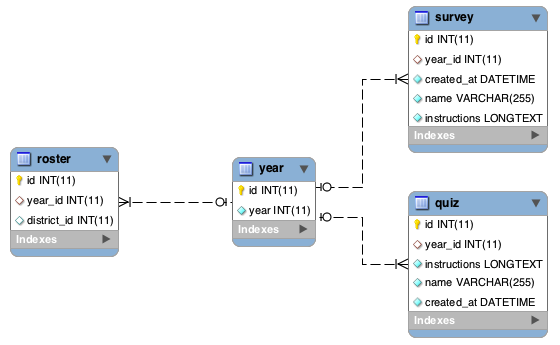
\includegraphics[width=0.7\textwidth]{figures/er/year}
	}
	\caption{Year Enhanced Entity-Relationship (EER) Diagram}
	\label{fig:er-year}
\end{figure}

We see in Figure \ref{fig:er-year}, that the year entity appropriately maintains a one-to-many relationship with each of the tables that reference it. In an EER diagram such as this, each box represents a table in a database and each row in a box corresponds to a column in that table. A connecting line indicates that a relationships exists between its connected tables. If we take the relationship between the year and survey tables as an example, the line, which is drawn using Crow's Foot notation, indicates that a survey can be given during one year and that a year can have many surveys given during it. This diagram additionally indicates that many quizzes (see Section \ref{subsec:design-quiz}) and many rosters (see Section \ref{subsec:design-district}) can also only be associated with only one year.

The user's choice of which year they want to have as their current context for data viewing and manipulation will have to persist between each page of the Collaborative Environment. Having to constantly select what year to interact . Therefore, once a user initially visits the web site, a PHP session variable will be established that tracks the year they select which will then be used by subsequent SQL queries to retrieve the requested data.

\subsubsection{Implementation}
As established in the previous section, the selected year must be persisted from page-to-page as well as be accessible in such a way that it will not require a user to constantly have to interact with a selector.

This was implemented by having a year selector list appear in the upper-right corner of each page in the Collaborate Environment, as shown in Figure \ref{fig:screens-year}. The list is populated by making an asynchronous HTTP GET request to the URL \texttt{/year} which will both provide all available academic years that have been configured and indicate which is the current year as selected by the user.

\begin{figure}[h!]
	\centering
	\fbox{
		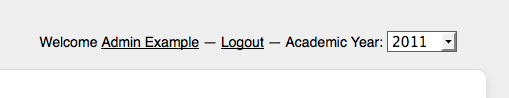
\includegraphics[width=0.6\textwidth]{figures/screens/year}
	}
	\caption{Year Selector Highlight}
	\label{fig:screens-year}
\end{figure}

Upon choosing a year from the selection, if it differs from the currently selected year, then an HTTP POST request will be sent to \texttt{/year/change/\textit{selected-year}}. This will cause the year PHP session variable to be updated to \emph{selected-year}. If the server responds with a success message, then the current web page will be refreshed and any changes to the data that are dependent on the year will be reflected.

%%%% Users
\subsection{User Management}
\label{subsec:design-user}
A User entity is perhaps the most fundamental object in the Collaborative Environment.  Users of each class, as defined in Section \ref{sec:overview-user-classes}, with the exception of anonymous, will be required to have an account with this system, and that account is what the User entity represents. The set of users minus anonymous will be referred to as ``registered users''.

	This entity facilitates the fulfillment of the Collaborative Environment's goal of logging user data by allowing the storage of a student's personal data such as gender, ethnicity, if they've graduated, and what college they are attending, in addition to student educational data such as standardized test scores, courses enrolled in, and after-school activities.

The collaborative functionality of the system also requires a User entity. Quiz attempts, survey submissions, and messaging need a way of differentiating one user from another.

\subsubsection{Design}
The Collaborative Environment internally refers to the set of user classes as ``roles''. Roles are easily stored in the database by using a role table such that its \emph{name} is stored in a column. The User entity, as modeled in Figure \ref{fig:er-user} stores two types of data: required information that applies to all registered users and personal/educational data that applies strictly to students. Required information consists of a user's \emph{username}, \emph{password}, \emph{salt}, \emph{firstName}, and \emph{lastName}.

\begin{figure}[h!]
	\centering
	\fbox{
		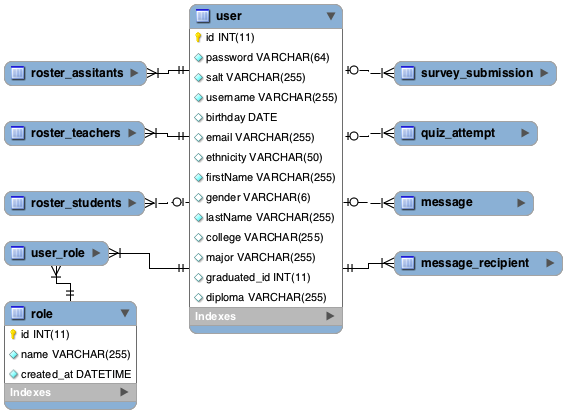
\includegraphics[width=0.7\textwidth]{figures/er/user}
	}
	\caption{User and Role EER Diagram}
	\label{fig:er-user}
\end{figure}

Each of these attributes has an obvious use except, perhaps, for \emph{salt} which is a precautionary security measure. All user passwords are hashed using using the SHA-256 cryptographic hash function. This means that if two users had the same password, then they would obviously result in identical hashes. This fact can be used exploited by people that have large masses of precomputed hashes. A salt, which is a randomly generated string, is append to the plaintext of a password before it is hashed. Now, even if the user's password is something common, what is hashed is, most likely, something unique.

For the sake of simplicity, we decided that the personal/education attributes \emph{birthday}, \emph{email}, \emph{ethnicity}, \emph{gender}, \emph{college}, \emph{major}, \emph{diploma}, and \emph{graduated} as year-independent data. This means that if and when these attributes have a value, that it will not vary based on what academic year the client has selected to be the current year; their values will persist through all years. On the other hand, there is strictly educational data that we do treat as year-dependent: activities, courses, exams, and grade level.

\begin{figure}[h!]
	\centering
	\fbox{
		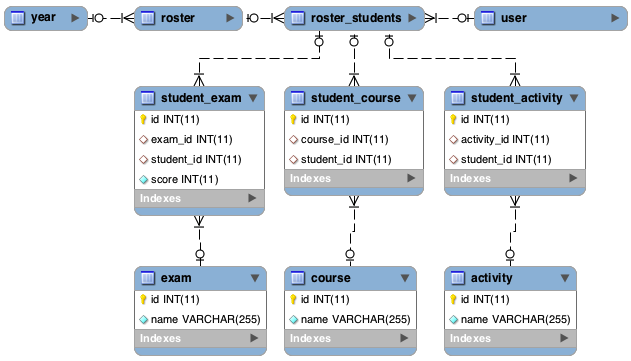
\includegraphics[width=0.7\textwidth]{figures/er/user-student}
	}
	\caption{Student user EER Diagram}
	\label{fig:er-user-student}
\end{figure}

Figure \ref{fig:er-user-student}, outlines the general model to achieve a year-dependent relationship between a student and their educational data and will be explained in depth in Section \ref{subsec:design-district}. Any given year is associated with many rosters, each of which contain a set of students in varying grade levels. Each student in a roster can then be associated with many exams, courses, and activities. 

\subsubsection{Implementation}
test

\begin{figure}[h!]
	\centering
	\setlength\fboxsep{0pt}
	\fbox{
		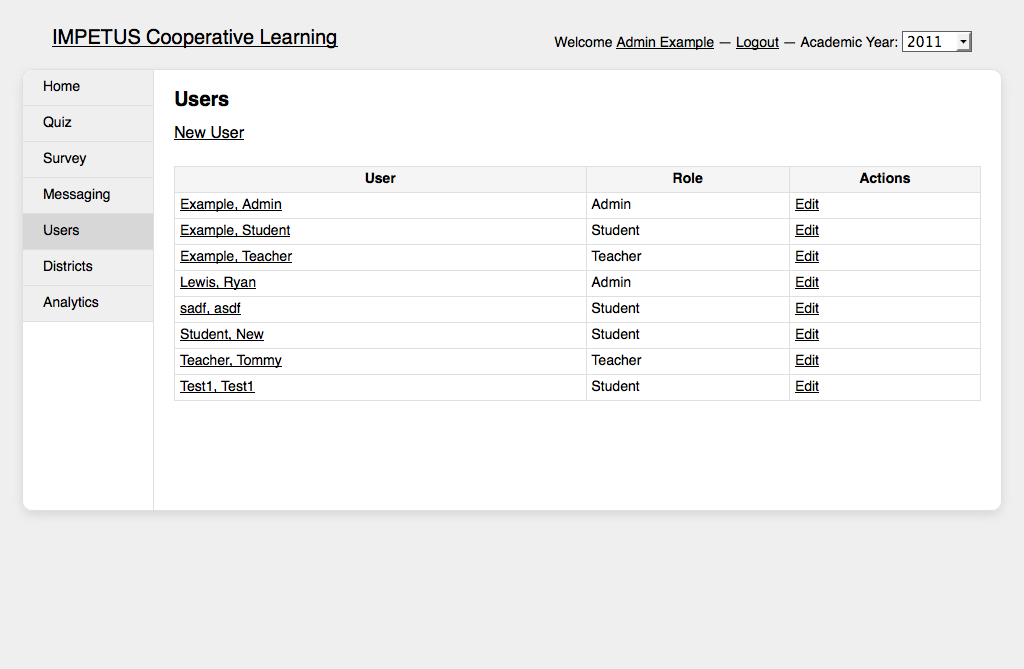
\includegraphics[width=0.8\textwidth]{figures/screens/user-list}
	}
	\caption{An privileged user's view of all the system's users.}
	\label{fig:screens-user-lust}
\end{figure}



\begin{figure}[h!]
	\centering
	\setlength\fboxsep{0pt}
	\fbox{
		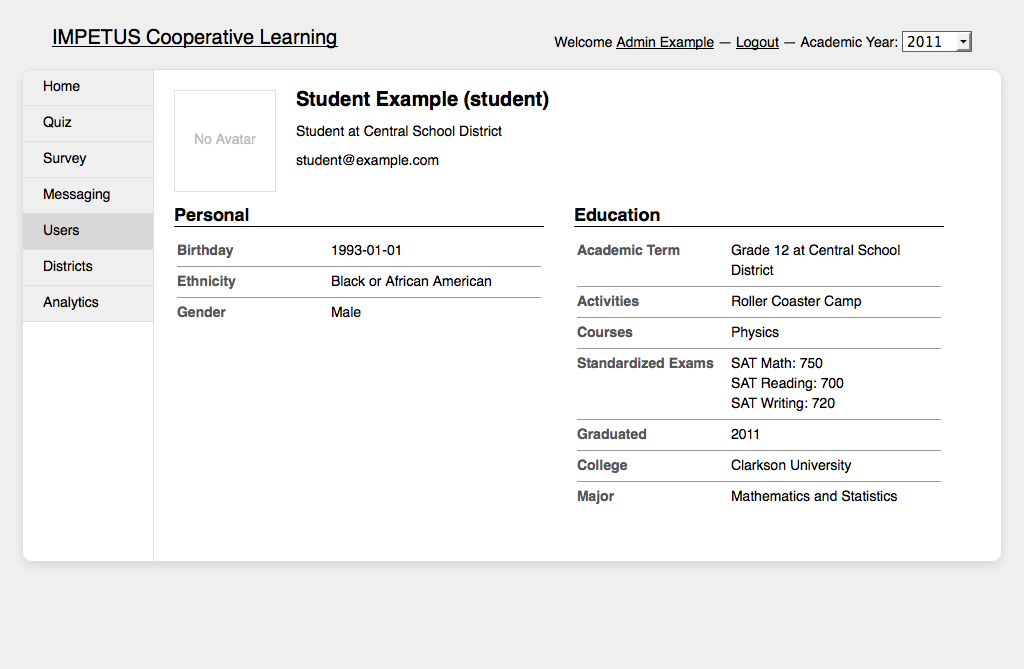
\includegraphics[width=0.8\textwidth]{figures/screens/user-student-profile}
	}
	\caption{A privileged user's view of a student's profile.}
	\label{fig:screens-user-student-profile}
\end{figure}



\begin{figure}[h!]
	\centering
	\setlength\fboxsep{0pt}
	\fbox{
		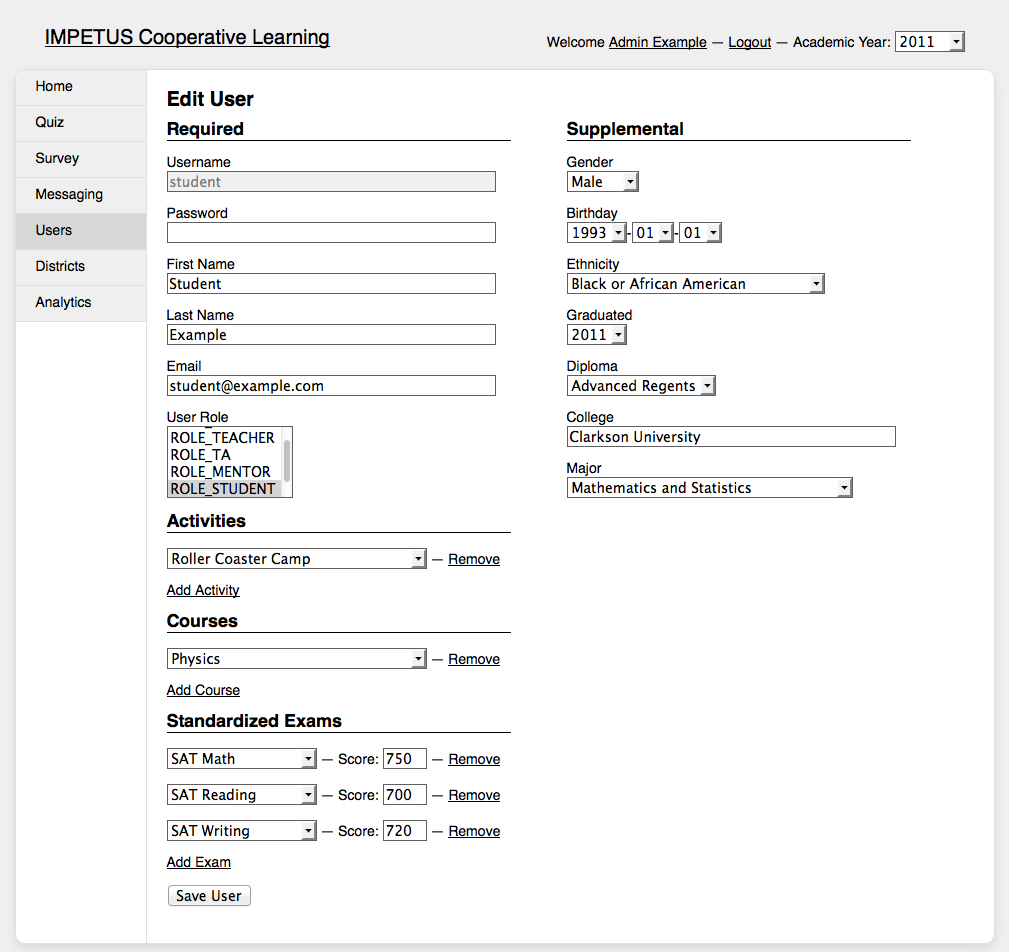
\includegraphics[width=0.8\textwidth]{figures/screens/user-student-edit}
	}
	\caption{A privileged user editing a student's account.}
	\label{fig:screens-user-student-edit}
\end{figure}



%%%% Districts
\subsection{District Management}
\label{subsec:design-district}
test

%%%% Quiz
\subsection{Quiz System}
\label{subsec:design-quiz}
test

%%%% Survey
\subsection{Survey System}
\label{subsec:design-survey}
test

%%%% Messaging
\subsection{Messaging}
\label{subsec:design-messaging}
test

%%%% Analytics
\subsection{Analytics}
\label{subsec:design-analytics}
test

\section{Known Issues}
\chapter{User Survey}
\label{chap:usability}

\section{Study Goals}

\section{Participants}

\section{Procedure}

\section{Results}

\begin{table}
\centering
\small{
\begin{tabular}{| L{8cm} |p{0.7cm}|p{0.7cm}|p{0.7cm}|p{0.7cm}|p{0.7cm}|p{0.7cm}|p{0.7cm}|}
	\multicolumn{1}{c}{Question} &
	\multicolumn{1}{c}{
		\begin{rotate}{45}
			Disagree Strongly
		\end{rotate}
	} &
	\multicolumn{1}{c}{
		\begin{rotate}{45}
			Disagree Somewhat
		\end{rotate}
	} &
	\multicolumn{1}{c}{
		\begin{rotate}{45}
			Disagree
		\end{rotate}
	} &
	\multicolumn{1}{c}{
		\begin{rotate}{45}
			Neither
		\end{rotate}
	} &
	\multicolumn{1}{c}{
		\begin{rotate}{45}
			Agree
		\end{rotate}
	} &
	\multicolumn{1}{c}{
		\begin{rotate}{45}
			Agree Somewhat
		\end{rotate}
	} &
	\multicolumn{1}{c}{
		\begin{rotate}{45}
			Agree Strongly
		\end{rotate}
	} \\ \hline
\hline Logging in is too complex.
	& \textbf{67\% \newline (12)} & 11\% \newline (2) & 6\% \newline (1) & 11\% \newline (2) & 6\% \newline (1) & - & - \\
\hline Switching between Academic Years is easy.
	& 11\% \newline (2) & - & - & 6\% \newline (1) & 6\% \newline (1) & 22\% \newline (4) & \textbf{56\% \newline (10)} \\
\hline Navigating to the User editor is easy.
	& 6\% \newline (1) & - & - & 22\% \newline (4) & 6\% \newline (1) & 22\% \newline (4) & \textbf{44\% \newline (8)} \\
\hline I intuitively knew how to add a Course and a Standardized Exam score to a User.
	& 6\% \newline (1) & - & - & 17\% \newline (3) & - & \textbf{50\% \newline (9)} & 28\% \newline (5) \\
\hline Students can be added to the system easily.
	& 6\% \newline (1) & - & - & 11\% \newline (2) & 11\% \newline (2) & 22\% \newline (4) & \textbf{50\% \newline (9)} \\
\hline Students can easily be added to a District's roster.
	& 6\% \newline (1) & - & 6\% \newline (1) & 22\% \newline (4) & 22\% \newline (4) & 11\% \newline (2) & \textbf{33\% \newline (6)} \\
\hline I find Districts to be confusing.
	& \textbf{44\% \newline (8)} & 6\% \newline (1) & 6\% \newline (1) & 22\% \newline (4) & 17\% \newline (3) & - & 6\% \newline (1) \\
\hline It is easy to add recipients to a message
	& - & - & 6\% \newline (1) & 11\% \newline (2) & 17\% \newline (3) & 11\% \newline (2) & \textbf{56\% \newline (10)} \\
\hline The messaging system is intuitive.
	& - & - & 6\% \newline (1) & 17\% \newline (3) & 6\% \newline (1) & 22\% \newline (4) & \textbf{50\% \newline (9)} \\
\hline Creating a Survey is confusing.
	& \textbf{39\% \newline (7)} & 17\% \newline (3) & 33\% \newline (6) & 6\% \newline (1) & 6\% \newline (1) & - & - \\
\hline Creating a Quiz is confusing.
	& 17\% \newline (3) & 6\% \newline (1) & 22\% \newline (4) & \textbf{28\% \newline (5)} & 11\% \newline (2) & 11\% \newline (2) & 6\% \newline (1) \\
\hline
\end{tabular}
}
\caption{Survey Agreement Questions and Results}
\label{table:agreement}
\end{table}

test

\begin{table}
\centering
\small{
\begin{tabular}{| L{8cm} |p{0.7cm}|p{0.7cm}|p{0.7cm}|p{0.7cm}|p{0.7cm}|}
\multicolumn{1}{c}{Question} &
	\multicolumn{1}{c}{
		\begin{rotate}{45}
			Grade 9
		\end{rotate}
	} &
	\multicolumn{1}{c}{
		\begin{rotate}{45}
			Grade 10
		\end{rotate}
	} &
	\multicolumn{1}{c}{
		\begin{rotate}{45}
			Grade 11
		\end{rotate}
	} &
	\multicolumn{1}{c}{
		\begin{rotate}{45}
			Grade 12
		\end{rotate}
	} &
	\multicolumn{1}{c}{
		\begin{rotate}{45}
			Unsure
		\end{rotate}
	} \\ \hline
\hline What grade is Sally in during Academic Year 2010?
	& - & - & \textbf{83\% \newline (15)} & 11\% \newline (2) & 6\% \newline(1) \\
\hline
\end{tabular}
}
\caption{Results of a test to see if year switching is accomplishable; Grade 11 is correct.}
\label{table:year}
\end{table}

test

\begin{table}
\centering
\small{
\begin{tabular}{| L{8cm} |p{0.7cm}|p{0.7cm}|p{0.7cm}|p{0.7cm}|p{0.7cm}|p{0.7cm}|p{0.7cm}|}
	\multicolumn{1}{c}{How satisfied are you with ... ?} &
	\multicolumn{1}{c}{
		\begin{rotate}{45}
			Extremely dissatisfied
		\end{rotate}
	} &
	\multicolumn{1}{c}{
		\begin{rotate}{45}
			Dissatisfied
		\end{rotate}
	} &
	\multicolumn{1}{c}{
		\begin{rotate}{45}
			Neither
		\end{rotate}
	} &
	\multicolumn{1}{c}{
		\begin{rotate}{45}
			Satisfied
		\end{rotate}
	} &
	\multicolumn{1}{c}{
		\begin{rotate}{45}
			Extremely satisfied
		\end{rotate}
	} \\ \hline
\hline The live user search feature
	& 6\% \newline (1) & 6\% \newline (1) & 22\% \newline (4) & 28\% \newline (5) & \textbf{39\% \newline (7)} \\
\hline The types of data that the Survey Results provides you with
	& - & 11\% \newline (2) & 17\% \newline (3) & \textbf{56\% \newline (10)} & 17\% \newline (3) \\
\hline The types of data that the Quiz Results provides you with
	& - & 6\% \newline (1) & \textbf{50\% \newline (9)} & 33\% \newline (6) & 11\% \newline (2) \\
\hline User creation
	& - & - & 11\% \newline (2) & 33\% \newline (6) & \textbf{56\% \newline (10)} \\
\hline User editing
	& - & - & 11\% \newline (2) & 33\% \newline (6) & \textbf{56\% \newline (10)} \\
\hline District editing
	& - & 6\% \newline (1) & 22\% \newline (4) & 22\% \newline (4) & \textbf{50\% \newline (9)} \\
\hline Messaging
	& - & - & 17\% \newline (3) & 39\% \newline (7) & \textbf{44\% \newline (8)} \\
\hline Survey creation
	& - & - & 17\% \newline (3) & \textbf{56\% \newline (10)} & 28\% \newline (5) \\
\hline Survey results
	& - & - & 17\% \newline (3) & 44\% \newline (8) & 39\% \newline (7) \\
\hline Quiz creation
	& - & 11\% \newline (2) & \textbf{33\% \newline (6)} & \textbf{33\% \newline (6)} & 22\% \newline (4) \\
\hline Quiz results
	& - & 6\% \newline (1) & 28\% \newline (5) & \textbf{44\% \newline (8)} & 22\% \newline (4) \\
\hline Overall system
	& - & - & 11\% \newline (2) & \textbf{61\% \newline (11)} & 28\% \newline (5) \\
\hline
\end{tabular}
}
\caption{Survey Satisfaction Questions and Results}
\label{table:satisfaction}
\end{table}

test
\chapter{Conclusions}
\label{chap:conclusion}

\section{Conclusions}
The primary contribution of this work is a free and open source web-based Collaborative Environment that ultimately provides a means of satisfying the STEP priorities and requirements by way of aiding in overcoming the issues of operating a geographically isolated STEM outreach program. By basing the Collaborative Environment on state-determined criteria, it can be utilized by any STEP funded institution that has a desire to provide web-based collaborative learning to its participants. Additionally, its open source nature allows for local customization and adoption for state programs outside of New York which have goals similar to that of STEP's. It has been shown that the currently implemented Collaborative Environment's feature set addresses the STEP priorities and requirements. Specifically:

\begin{description}
	\item [User Management] \hfill \\ The storage of student data is facilitated by this system. It allows for personal data, such as gender and ethnicity, and educational data, such as standardized test scores, courses enrolled in, and after-school activities participated in, to be stored on a yearly basis. This data can be used to show improvement in the STEP program priorities: the recruitment/retention rates of male users and underrepresented minorities as well as tracking NYS Math and Science assessment examination scores.
	\item [Quiz System] \hfill \\ Allows coaches and teaching assistants to create quizzes to measure student performance and act as a supplemental educational tool during student collaborative and self-learning. Students can use these quizzes as a means of brushing up on topics they are struggling with, while teaching assistants can use quizzes as a way to ensure their students are learning. This system assists in the fulfillment of the STEP program requirements stating that there must be formal collaborations between the funded institute and the local school districts in addition to providing activities that will assist students in acquiring the skills and aptitudes necessary to pursue collegiate STEM disciplines.
	\item [Learning Pathway] \hfill \\ Using a visualization of state math standards in the form a hierarchical tree of dependencies, students can readily identify which topics they are proficient in and which they need assistance with. Each node in this tree represents a state standard and has associated with it both external video resources via the Khan Academy and quizzes created using the Quiz System. Nodes change color based on a student's performance on the quizzes so that a quick look at the tree will identify all the areas that an individual student does and does not need help with. This ability to know what students need help with on a individual and personalized basis via a tool backed by actual state standards will aid in accomplishing the STEP program requirement which states there must exist services to enhance the math and science skills in accordance with the Advanced Regent Diploma.
	\item [Survey System] \hfill \\ Coaches and teaching assistants can create surveys to be distributed to the Collaborative Environment's user base. This system can be used to gather valuable data and feedback from all of the participating bodies. Additionally, this can be used as a way to identify which students might need early intervention to keep them succeeding. If a user does not fill out a survey, it might be a sign that the student needs some additional attention.
	\item [Messaging] \hfill \\ Prior to the creation of this tool, there was no central resource for being able to communicate with any of the members of the IMPETUS program (students, coaches, assistants). Since all members will have an account (with an email address associated with it) in the Collaborative Environment, using a private message system which also notifies recipients that they have new mail is ideal for maintaining connections and collaboration.
\end{description}

Since the Collaborative Environment is open source and built using a set of well-defined existing tools, such as Symfony and Google Maps, it is a reasonably sustainable application for future work and maintenance. A future maintainer would have to be familiar with the concepts described in \S \ref{subsec:design-background-symfony}, SQL and database modeling, and object-oriented programming in PHP. Expected annual upkeep entails creating a new academic year, transitioning each district's roster to the newly created academic year, and ensuring that the standards-based learning pathway is accurate.

Additionally, a user survey was performed to gather some initial feedback regarding the Collaborative Environment. Although a lot of helpful comments were received, it is important to remember that the user study experiment was only run once and had a limited number of responses (18). Therefore, the qualitative responses that were received could not be used to concretely assert facts regarding the Collaborative Environment's usability. That being said, in an anecdotal sense, the results of this initial research have been primarily positive with 89\% of the participants indicating satisfaction with the system.

\section{Future Work}
There exist several areas of future work for this project:
\begin{itemize}
	\item The Analytics feature discussed in \S \ref{subsec:design-analytics} was designed to make completing the annual STEP summary report easier by formatting the data collected by the Collaborative Environment into that expected by the report. As of the current implementation, only 4 of the 16 data tables required by the annual report are generated.
	\item Conduct another usability study to obtain qualitative data regarding the redesigned features based on the first usability study. Once another usability test has been administered, it can be compared to the one presented in this paper to have quantitative data indicating, for instance, an improvement between designs. Future studies must involve IMPETUS tutors, mentors, and students as they were a missed in the initial one.
	\item Due to the Collaborative Environment's data logging capabilities, it can be used as a powerful research tool. For example, student quiz results for multiple academic years can be analyzed to determine which quiz questions resulted in different levels of student academic achievement.
	\item The open source nature of the Collaborative Environment allows it to be potentially utilized by other STEP programs. Making these other programs aware of its existence could lead to better software and, consequently, better STEP programs by building a community around the Collaborative Environment. Additionally, reaching out to the Khan Academy could lead to a mutually beneficial exchange of information regarding collaborative and educational software.
\end{itemize}
% End chapters

\singlespacing

\raggedright
\bibliography{bibliography/bibliography}
\bibliographystyle{plain}

\doublespacing

\begin{appendices}
%\chapter{User Manual}

\chapter{Administrator Manual}
\chapter{Analytical Data Screenshots}
\label{chap:analytical-appendix}

\begin{figure}[h!]
	\centering
	\fbox{
		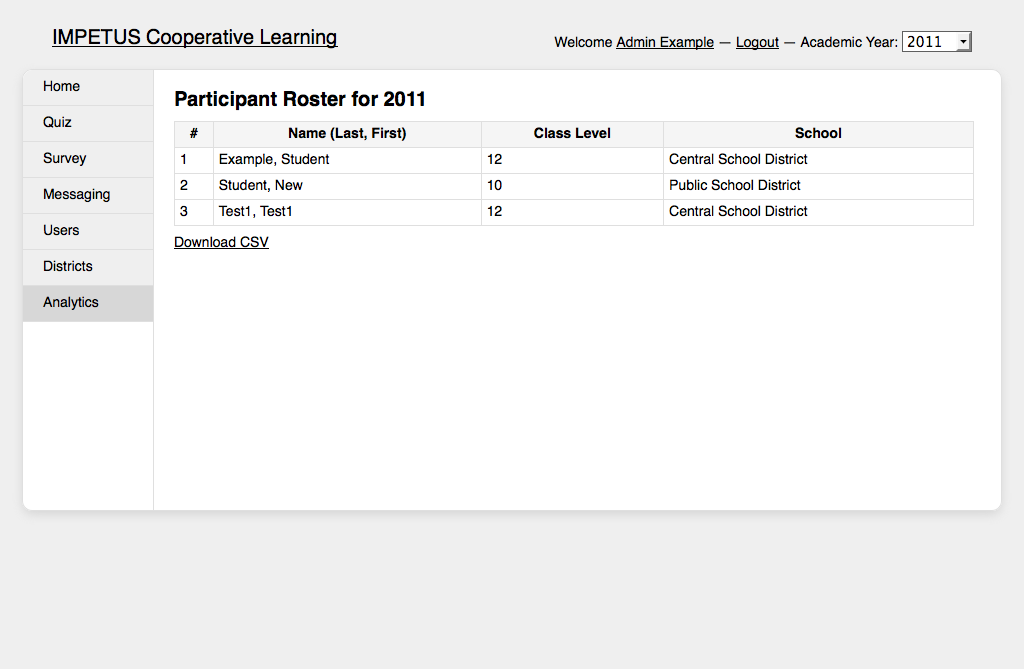
\includegraphics[width=0.8\textwidth]{figures/screens/analytics/analytics-participants}
	}
	\caption{Sample listing of all STEP student participants.}
	\label{fig:screens-analytics-participants}
\end{figure}

\begin{figure}[h!]
	\centering
	\fbox{
		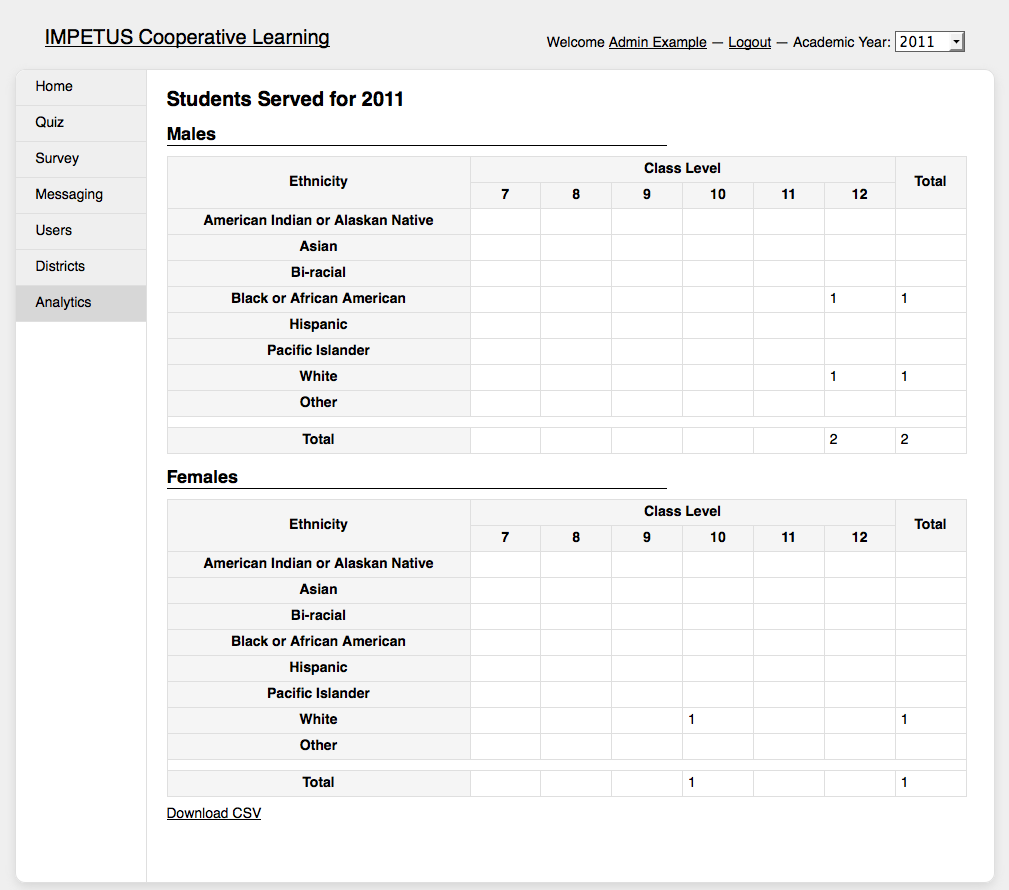
\includegraphics[width=0.8\textwidth]{figures/screens/analytics/analytics-students}
	}
	\caption{Sample listing of the number of students of each ethnicity in grades 7-12 grouped by gender.}
	\label{fig:screens-analytics-students}
\end{figure}

\begin{figure}[h!]
	\centering
	\fbox{
		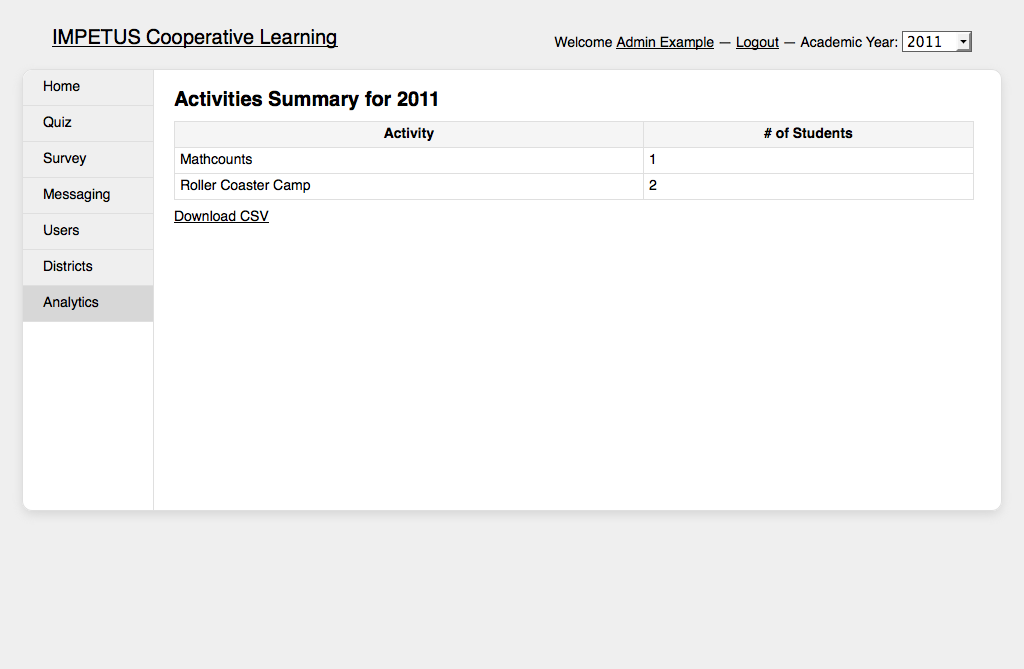
\includegraphics[width=0.8\textwidth]{figures/screens/analytics/analytics-activities}
	}
	\caption{Sample listing of the number of students participating in each activity.}
	\label{fig:screens-analytics-activities}
\end{figure}

\begin{figure}[h!]
	\centering
	\fbox{
		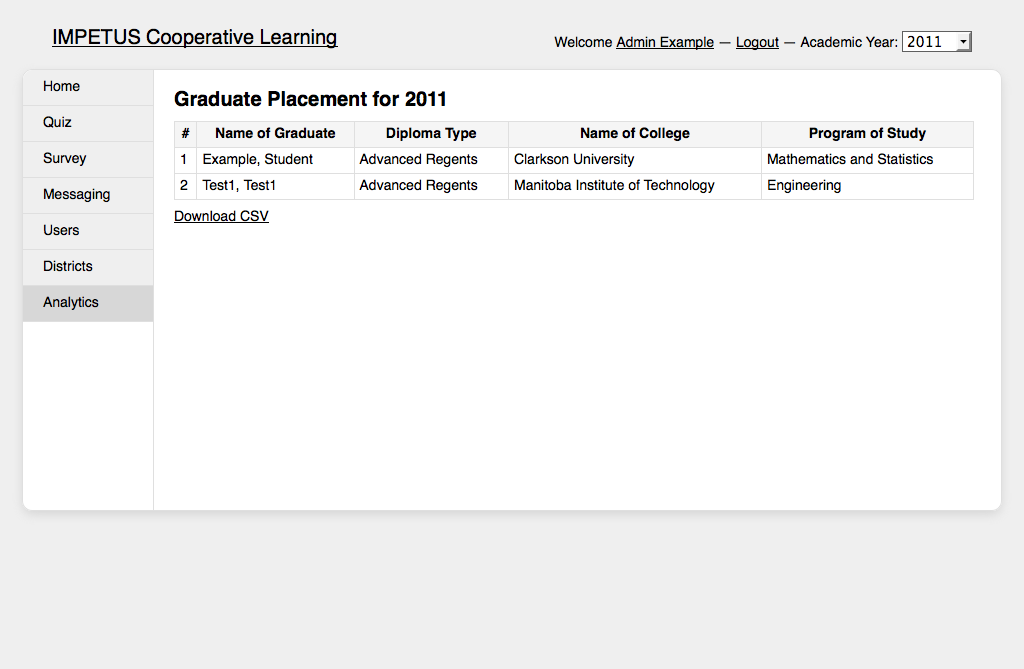
\includegraphics[width=0.8\textwidth]{figures/screens/analytics/analytics-graduates}
	}
	\caption{Sample listing of each graduating student and details of the college they will attend.}
	\label{fig:screens-analytics-graduates}
\end{figure}

\end{appendices}

\end{document}
